\begin{figure}[tbp]
\centering
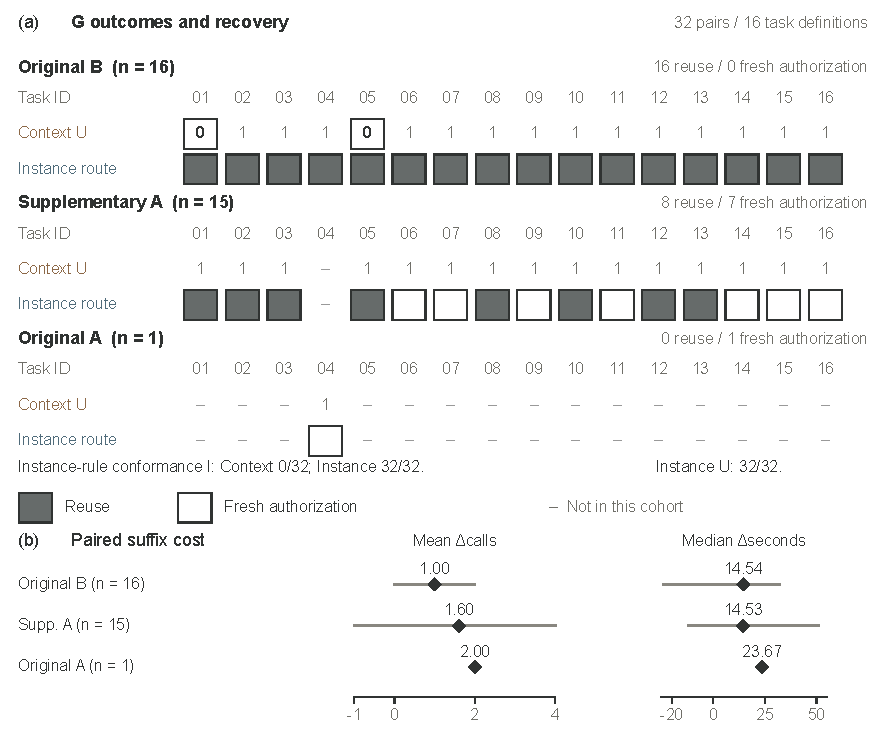
\includegraphics[width=\linewidth]{figures/fig5-recovery-cost.pdf}
\caption{All 32 delivered G pairs across 16 task definitions. (a) Task columns align across cohorts; dashes mean absent from that cohort's delivered pairs, not failure. Supplementary A omits 04; Original A includes only 04. $I$ denotes instance-rule conformance, not safety under the context policy. Context has $I=0$ throughout and $U=1$ in 30 pairs; all bound arms end with $U=1,I=1$. Filled/open squares denote reuse/fresh authorization. (b) Diamonds show mean call and median elapsed-time differences for complete paired suffixes ($\Delta=$ bound minus context); segments show observed minima--maxima, not confidence intervals. Time includes decisions, tool interactions and terminal paths. Table~\ref{tab:recovery-decomposition} separates recovery calls}
\label{fig:recovery}
\end{figure}
